%%%%%%%%%%%%%%%%%%%%%%%%%%%%%%%%%%%%%%%%%%%%%%%%%%%%%%%%%%%%%%%%%%%%%%%%%%%%%%%%
%%%%%%%%%%%%%%%%%%%%  Set document class, and configure it  %%%%%%%%%%%%%%%%%%%%
%%%%%%%%%%%%%%%%%%%%%%%%%%%%%%%%%%%%%%%%%%%%%%%%%%%%%%%%%%%%%%%%%%%%%%%%%%%%%%%%


% Define the document class
\documentclass[a4paper]{tufte-handout}

% Used for adding images/graphics to the document
\usepackage{graphicx}
  % Set default scaling for included graphics
  \setkeys{Gin}{width=\linewidth,totalheight=\textheight,keepaspectratio}
  % Define base path for graphics, change this as needed
  \graphicspath{{graphics/}}

% Improves the quality of tables in LaTeX
% It provides useful commands, and ads some behind the scenes optimizations
% Tables created by this package are similar to the tables in Tufte's books
\usepackage{booktabs}

% Provides a way to set units in typographically correct way
% It includes the `nicefrac' package to provide nicer looking fractions
% Common commands include \unit[<value>]{<unit>}, \nicefrac{<num>}{<den>},
% and \unitfrac[<value>]{<num>}{<den>}
% The \nicefrac can take a font command as an optional argument
\usepackage{units}

% Extends verbatim with new environments, and more features
\usepackage{fancyvrb}
  % Sets default verbatim font, smaller than default
  \fvset{fontsize=\small}

% Changes how the date is displayed in the document,
% and provides extra date related commands
% I prefer the ISO format yyyy-mm-dd, but it can be changed as needed
% Also used to print <month> <year> in the copyright page
\usepackage[style=iso,en-US]{datetime2}

% Can enable or disable hyphenation of words, even in TT font environments
\usepackage[htt]{hyphenat}


%%%%%%%%%%%%%%%%%%%%%%%%%%%%%%%%%%%%%%%%%%%%%%%%%%%%%%%%%%%%%%%%%%%%%%%%%%%%%%%%
%%  Define document metadata, and other useful things like bibliography file  %%
%%%%%%%%%%%%%%%%%%%%%%%%%%%%%%%%%%%%%%%%%%%%%%%%%%%%%%%%%%%%%%%%%%%%%%%%%%%%%%%%


\title{An Example of the Tufte-Handout Style\thanks{Inspired by Edward Tufte!}}
\author[The Tufte-LaTeX Developers]{The Tufte-\LaTeX\ Developers}
%\date{2025-01-28} % If the \date command is omitted, current date will be used

% Debugging
%\geometry{showframe} % display margins for debugging page layout

% Define BibLaTeX resource file
\addbibresource{sample-bibliography.bib}


%%%%%%%%%%%%%%%%%%%%%%%%%%%%%%%%%%%%%%%%%%%%%%%%%%%%%%%%%%%%%%%%%%%%%%%%%%%%%%%%
%%%%%%  These can be removed in actual documents, only used for examples  %%%%%%
%%%%%%%%%%%%%%%%%%%%%%%%%%%%%%%%%%%%%%%%%%%%%%%%%%%%%%%%%%%%%%%%%%%%%%%%%%%%%%%%


% This package allows for easy insertion of dummy text
\usepackage[language=english]{lipsum}

% Tries to intuit whether or not to add a space after a command
% Used in some documentation commands here, but can be used in other places as well
\usepackage{xspace}

% This package lets writer include fancy TeX logos in text
\usepackage{hologo}

% Shortcuts for printing Tufte's book titles
% The lowercase commands will produce the initials of the book title in italics
% The all-caps commands will print out the full title of the book in italics
% Uses xspace to add a space after the command unless it's followed by punctuation
\newcommand{\vdqi}{\textit{VDQI}\xspace}
\newcommand{\ei}{\textit{EI}\xspace}
\newcommand{\ve}{\textit{VE}\xspace}
\newcommand{\be}{\textit{BE}\xspace}
\newcommand{\VDQI}{\textit{The Visual Display of Quantitative Information}\xspace}
\newcommand{\EI}{\textit{Envisioning Information}\xspace}
\newcommand{\VE}{\textit{Visual Explanations}\xspace}
\newcommand{\BE}{\textit{Beautiful Evidence}\xspace}

% Shortcut for printing the Tufte-LaTeX class name
\newcommand{\TL}{Tufte-\hologo{LaTeX}\xspace}

% Shortcuts for printing various TeX logos and adding them into the index
% Prints formatted XeLaTeX logo and adds it to the index
\newcommand{\iXeLaTeX}{\hologo{XeLaTeX}\index{XeLaTeX@\protect\hologo{XeLaTeX}}\xspace}
% Prints formatted LuaLaTeX logo and adds it to the index
\newcommand{\iLuaLaTeX}{\hologo{LuaLaTeX}\index{LuaLaTeX@\protect\hologo{LuaLaTeX}}\xspace}
% Prints formatted pdfLaTeX logo and adds it to the index
\newcommand{\iPdfLaTeX}{\hologo{pdfLaTeX}\index{pdfLaTeX@\protect\hologo{pdfLaTeX}}\xspace}
% Prints formatted BibLaTeX logo and adds it to the index
\newcommand{\iBibLaTeX}{Bib\hologo{LaTeX}\index{BibLaTeX@\protect{}Bib\hologo{LaTeX}}\xspace}

% Prints a TODO item in bold tufte-red color, followed by the text of the TODO item
\newcommand{\TODO}[1]{\textcolor{tufte-red}{\textbf{TODO!} #1}\xspace}

% Used to print LaTeX commands with normalized font styles and environments
% Highlights text in tufte-orange color
\newcommand{\hlorange}[1]{\textcolor{tufte-orange}{#1}}
% Print command in mono font, in hlorange color, with backlash
\newcommand{\doccmd}[1]{\hlorange{\texttt{\textbackslash#1}}}
% Print an optional command argument, italicised, serif font, in angle brackets
\newcommand{\docopt}[1]{\( \langle \)\textrm{\textit{#1}}\( \rangle \)}
% Print a required command argument, italicised, serif font
\newcommand{\docarg}[1]{\textrm{\textit{#1}}}
% Print environment, in mono font, in hlorange color
\newcommand{\docenv}[1]{\hlorange{\texttt{#1}}}
% Print package name, in mono font, in hlorange color
\newcommand{\docpkg}[1]{\hlorange{\texttt{#1}}}
% Print class name, in mono font
\newcommand{\doccls}[1]{\texttt{#1}}
% Print document class option, in mono font, in hlorange color
\newcommand{\docclsopt}[1]{\hlorange{\texttt{#1}}}
% Print file hook (customization file), in mono font
\newcommand{\docfilehook}[1]{\texttt{#1}}
% Environment for command specification, uses mono font, no skips or indents
\newenvironment{docspec}
  % Define start of the environment
  {\begin{quotation}\ttfamily\parskip0pt\parindent0pt\ignorespaces}
  % Define end of the environment
  {\end{quotation}}


%%%%%%%%%%%%%%%%%%%%%%%%%%%%%%%%%%%%%%%%%%%%%%%%%%%%%%%%%%%%%%%%%%%%%%%%%%%%%%%%
%%%%%%%  Main handout contents follow from here, add your document here  %%%%%%%
%%%%%%%%%%%%%%%%%%%%%%%%%%%%%%%%%%%%%%%%%%%%%%%%%%%%%%%%%%%%%%%%%%%%%%%%%%%%%%%%


\begin{document}

% Print title with author and date
\maketitle

% Add an abstract
\begin{abstract}
  \noindent
  This document describes the \TL\ \doccls{tufte-handout} document class style.
  It also provides examples and comments on the style's use.
  Only a brief overview is presented here;  for a complete reference, see the sample book.

  As mentioned in the sample book, some of the changes done in the \TL\ classes are not in spirit with Tufte's designs.
  The changes were made to make the produced documents more accessible to my personal needs and preferences.
  However I have done my best to provide a way of disabling or easily overwriting these changes.
\end{abstract}


\section{\TL\ Design}\label{sec:tufte-latex-design}
The \TL\ document classes define a style similar to the style Edward Tufte uses in his books and handouts.
Tufte's style is known for its extensive use of sidenotes, tight integration of graphics with text, and well-set typography.
This document aims to be at once a demonstration of the features of the \TL\ document classes and a style guide to their use.

\subsection{Headings}\label{sec:headings}
This style provides \textsc{a}- and \textsc{b}-heads (that is, \doccmd{section} and \doccmd{subsection}), demonstrated above.
\paragraph{Paragraph} The \doccmd{paragraph} headings (as shown here) are introduced by italicized text and separated from the main paragraph by a bit of space.

By default \doccmd{subsubsection} and \doccmd{subparagraph} headings are not defined in the \TL\ classes.
They will emit an error if you try to use them and any smaller heading.
For more information about these choices, see the sample book for subsection called \textit{``Headings''} in the \textit{``On the Use of the \texttt{tufte-book} Document Class''} chapter.
There is also an informative section called \textit{``Numbered Section Headings''} in the \textit{``Customizing \TL''} chapter.

% Start a new thought which will put text in caps and give it a bit of vertical space
% Note how the citation is placed in the margin as a sidenote
\newthought{In his later books},\cite{Tufte2006} Tufte starts each section with a ``new thought''.
It has bit of vertical space, a non-indented paragraph, and sets the first few words in \textsc{small caps}.
To accomplish this effect using this style, use the \Verb|\newthought| command:
\begin{docspec}
  \doccmd{newthought\{In his later books\}, Tufte starts\ldots}
\end{docspec}

\subsection{Sidenotes}\label{sec:sidenotes}
One of the most prominent and distinctive features of this style is the extensive use of sidenotes.
The wide margin on the right side provides ample room for sidenotes and small figures.
Any \doccmd{footnote} will automatically be converted into a \doccmd{sidenote}.%
\footnote{This is a sidenote that was entered using the \doccmd{footnote} command.}
If you'd like to place ancillary information in the margin without the sidenote mark (the superscript
number), you can use the \doccmd{marginnote} command.
\marginnote{%
  This is a margin note.
  Notice that there isn't a number preceding the note, and there is no number in the main text where this note was written.
}

In his books Tufte places margin on the right side of the page, regardless whether it's an even or odd page.
If you prefer to alternate the placement of margins, so they fall on outer edge you can use the \docclsopt{symmetric} class option.

\newthought{On a personal note}, placing of sidenotes---be it footnote, citation, or other---should follow the following rules:
\begin{itemize}
  \item If the sidenote applies to the whole sentence, it should be placed after the period or other punctuation mark.
  \item If the sidenote applies to a specific word, it should be placed immediately after that word, even if the word is in the middle of the sentence, or followed by a punctuation mark.
  \item If a sidenote is a complete sentence, or a citation, it should end with a period.
\end{itemize}
The specification of the \doccmd{sidenote} command is:
\begin{docspec}
  \doccmd{sidenote}[\docopt{number}][\docopt{offset}]\{\docarg{Sidenote text.}\}
\end{docspec}

Both the \docopt{number} and \docopt{offset} arguments are optional.
If you provide a \docopt{number} argument, then that number will be used as the sidenote number.
It will only change the number of the current sidenote, and will not affect the numbering sequence of subsequent sidenotes.

Sometimes a sidenote may run over the top of other text or graphics in the margin space.
If this happens, you can adjust the vertical position of the sidenote by providing a dimension in the \docopt{offset} argument.
Some examples of valid dimensions are:
\begin{docspec}
  \ttfamily 1.0in \qquad 2.54cm \qquad 254mm \qquad 6\Verb|\baselineskip|
\end{docspec}
If the dimension is positive, it will push the sidenote down the page; if the dimension is negative, it will pull the sidenote up the page.

While both the \docopt{number} and \docopt{offset} arguments are optional, they must be provided in order.
To adjust the vertical position of the sidenote while leaving the sidenote number alone, use the following syntax:
\begin{docspec}
  \doccmd{sidenote}[][\docopt{offset}]\{\docarg{Sidenote text.}\}
\end{docspec}
The empty brackets tell the \Verb|\sidenote| command to use the default sidenote number.

If you \emph{only} want to change the sidenote number, however, you may completely omit the \docopt{offset} argument:
\begin{docspec}
  \doccmd{sidenote}[\docopt{number}]\{\docarg{Sidenote text.}\}
\end{docspec}

The \doccmd{marginnote} command has a similar \docarg{offset} argument:
\begin{docspec}
  \doccmd{marginnote}[\docopt{offset}]\{\docarg{Margin note text.}\}
\end{docspec}

\subsection{References}
References are placed alongside their citations as sidenotes, as well.
This can be accomplished using the normal \doccmd{cite} command or the \doccmd{autocite} command, which functions similarly.%
\sidenote{%
  If you use the \doccmd{cite} command within a sidenote, it will render as an in-line parenthetical citation, as demonstrated here \autocite{Tufte2001}.
}

You will need to specify a bibliography resource file in the preamble of your document using \doccmd{addbibresource}\{\docarg{bibliography-file.bib}\} command.
The complete list of references may be printed automatically by using the \doccmd{printbibliography} command.
See the end of this document for an example, and the \iBibLaTeX\ documentation for more information.
Bibliography can be turned off with the help of \docclsopt{nobib} class option.

To enter multiple citations at one location,\autocite{Tufte2006,Tufte1990} you can provide a list of keys separated by commas: 
\begin{docspec}
  \doccmd{cite}\{\docarg{bibkey1,bibkey2,\ldots}\}
\end{docspec}

\newthought{In the new version of \TL}, it's impossible to offset citation's position the same way sidenotes can be moved up or down the margin.
This is caused by the change from \docpkg{natbib} package and \hologo{BibTeX} tool to \docpkg{biblatex} package and \hologo{biber} tool.
The \docpkg{biblatex} provides it own optional arguments for the \doccmd{cite} commands, which are kept unchanged to avoid confusion.
I see the possible breakage of old \TL\ documents as a fair tradeoff for the new features and flexibility that \docpkg{biblatex} provides.
It is worth noting that the \docpkg{natbib} is mostly kept on life support, so it's better to switch now and make \TL\ more maintainable in the future.
This is one of the reasons why this version of \TL\ classes has a new major version number.


\subsection{Figures and Tables}\label{sec:figures-and-tables}
Images and graphics play an integral role in Tufte's work.
In addition to the standard \docenv{figure} and \docenv{tabular} environments, this style provides special figure and table environments for full-width floats.

Full page-width figures and tables may be placed in \docenv{figure*} or \docenv{table*} environments.
To place figures or tables in the margin, use the \docenv{marginfigure} or \docenv{margintable} environments as follows (see \cref{fig:marginfig}):
\begin{marginfigure}%
  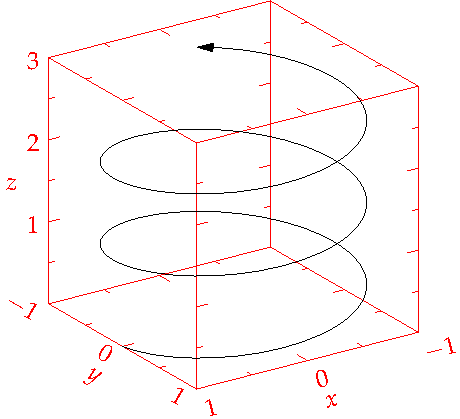
\includegraphics[width=\linewidth]{helix}
  \caption[This is an example of a margin figure]{%
    This is a margin figure. 
    The helix is defined by \(x = \cos(2\pi z)\), \(y = \sin(2\pi z)\), and \(z = [0, 2.7]\). 
    The figure was drawn using \href{http://asymptote.sf.net/}{Asymptote} (\url{http://asymptote.sf.net/}).
  }\label{fig:marginfig}
\end{marginfigure}
\noindent
\begin{Verbatim}
  \begin{marginfigure}
    \includegraphics{margin-figure}
    \caption{Margin figure caption}%
    \label{fig:margin-figure-label}
  \end{marginfigure}
\end{Verbatim}

The \docenv{marginfigure} and \docenv{margintable} environments accept an optional parameter \docopt{offset} that adjusts the vertical position of the figure or table. 
See the ``\nameref{sec:sidenotes}'' section above for examples of how to use offsets.
The specifications are:
\noindent
\begin{Verbatim}[commandchars=+/|]
  \begin{marginfigure}[+docopt/offset|] % or margintable
    +ldots
  \end{marginfigure}
\end{Verbatim}

\pagebreak
\Cref{fig:fullfig} is an example of the \docenv{figure*} environment and \cref{fig:textfig} is an example of the normal
\docenv{figure} environment.

\begin{figure*}[h]
  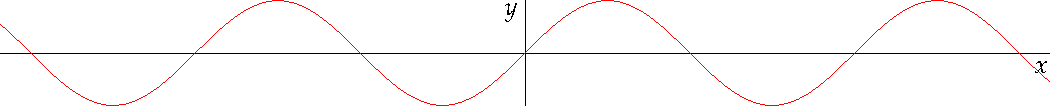
\includegraphics[width=\linewidth]{sine.pdf}%
  \caption[Sine graph showcasing full width figure environment]{%
    This graph shows \(y = \sin x\) from about \(x = [-10, 10]\).
    \emph{Notice that this figure takes up the full page width.}
  }\label{fig:fullfig}
\end{figure*}

\begin{figure}
  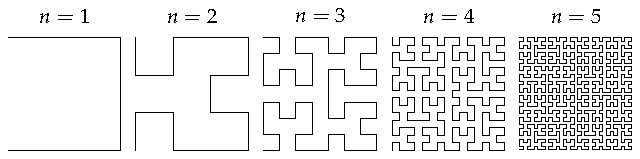
\includegraphics{hilbert-curves.pdf}
  \caption[Hilbert curves of various degrees \(n\)][2em]{%
    Hilbert curves of various degrees \(n\).
    \emph{Notice that this figure only takes up the main textblock width.}
  }\label{fig:textfig}
\end{figure}

\newthought{As with sidenotes and marginnotes}, a caption may require vertical adjustment. 
The \doccmd{caption} command can take a second optional argument which enables you to do this by providing a dimension \docopt{offset}.
You may specify the caption in any one of the following forms:
\begin{docspec}
  \doccmd{caption}\{\docarg{long caption}\} \\
  \doccmd{caption}[\docarg{short caption}]\{\docarg{long caption}\} \\
  \doccmd{caption}[][\docopt{offset}]\{\docarg{long caption}\} \\
  \doccmd{caption}[\docarg{short caption}][\docopt{offset}]\{\docarg{long caption}\}
\end{docspec}
A positive \docopt{offset} will push the caption down the page.
The short caption, if provided, is what appears in the list of figures/tables, otherwise the ``long'' caption appears there.
Note that although the arguments \docopt{short caption} and \docopt{offset} are both optional, they must be provided in order. 
Thus, to specify an \docopt{offset} without specifying a \docopt{short caption}, you must include the first set of empty brackets \Verb|[]|, which tell \doccmd{caption} to use the default ``long'' caption. 
As an example, the caption to \cref{fig:textfig} above was given in the form:
\begin{docspec}
  \doccmd{caption}[Hilbert curves\ldots][1em]\{Hilbert curves\ldots{}\}
\end{docspec}

\newthought{Note that caption offset is unavailable} for \docenv{marginfigure} and \docenv{margintable} environments.
In these cases you need to offset the whole figure or table.
Captions in \docenv{marginfigure} and \docenv{margintable} still support short captions.

\newthought{Tufte style tables are simple} and should be styled with the \docpkg{booktabs} package.
\Cref{tab:normaltab} shows table created with the \docpkg{booktabs} package.
Notice the lack of vertical rules---they serve only to clutter the table's data.
Hence Tufte style tables use only horizontal rules.
In cases where a table has many rows, \docpkg{colortbl} can be used to make rows stand out visually from each other.
Colors can be used to group related rows, highlight important data, or make one row stand out from the others.

\pagebreak
\begin{table}[ht]
  \centering
  \fontfamily{ppl}\selectfont
  \begin{tabular}{ll}
    \toprule
    Margin & Length \\
    \midrule
    Paper width               & \unit[8\nicefrac{1}{2}]{inches} \\
    Paper height              & \unit[11]{inches} \\
    Textblock width           & \unit[6\nicefrac{1}{2}]{inches} \\
    Textblock/sidenote gutter & \unit[\nicefrac{3}{8}]{inches} \\
    Sidenote width            & \unit[2]{inches} \\
    \bottomrule
  \end{tabular}
  \caption[Dimensions of the margins in \doccls{tufte-handout}]{%
  Here are the dimensions of the various margins used in the Tufte-handout class.%
  }\label{tab:normaltab}
\end{table}


\subsection{Too Many Floats}\label{ssec:too-many-floats}
\newthought{Occasionally} \hologo{LaTeX} will generate an error message:
\begin{docspec}
  Error: Too many unprocessed floats
\end{docspec}
\hologo{LaTeX} tries to place floats in the best position on the page.
Until it's finished composing the page, however, it won't know where those positions are.
If you have a lot of floats on a page (including sidenotes, margin notes, figures, tables, etc.),
\hologo{LaTeX} may run out of ``slots'' to keep track of them and will generate the aforementioned error.

\hologo{LaTeX} initially allocates 18 slots for storing floats. 
To work around this limitation, the \TL\ document classes provide a \doccmd{morefloats} command that will reserve more slots.

The first time \doccmd{morefloats} is called, it allocates an additional 34 slots.
The second time \doccmd{morefloats} is called, it allocates another 26 slots.

The \doccmd{morefloats} command may only be used two times.
Calling it a third time will generate an error message:
\begin{docspec}
  You may only call \string\morefloats\space twice\\
  See the Tufte-LaTeX documentation for alternatives
\end{docspec}
This is because allocating more floats may lead \hologo{LaTeX} to run out of memory.

If, after using the \doccmd{morefloats} command twice, you continue to get the \texttt{Too many unprocessed floats} error, there are a couple things you can do:

The \doccmd{FloatBarrier} command will immediately process all the floats before typesetting more material.
Since \doccmd{FloatBarrier} will start a new paragraph, you should place this command at the beginning or end of a
paragraph.

The \doccmd{clearpage} command will also process the floats before continuing, but instead of starting a new paragraph, it will start a new page.

You can also try moving your floats around a bit: move a figure or table to the next page, or reduce the number of sidenotes.
Keep in mind that each sidenote actually uses \emph{two} float slots.

After placing the floats, \hologo{LaTeX} will mark those slots as unused so they are available for the next page to be composed.


\subsection{Captions}
You may notice that the captions are sometimes misaligned.
Due to the way \hologo{LaTeX}'s floats works, it's hard to know for sure where it decided to put the float.
Therefore, the \TL\ document classes provide commands to override the caption position.

\paragraph{Vertical alignment}\label{par:vertical-alignment}
In cases where the caption is too high or too low on the page, you can adjust its vertical position.
To override the caption's vertical alignment, use the provided \doccmd{setfloatalignment} command inside the float environment.
For example:

\begin{Verbatim}[commandchars=+/|]
\begin{figure}
  \includegraphics{vertical-figure}
  \caption{vertical-figure-caption}%
  \label{fig:vertical-figure-label}
  +hlorange/\setfloatalignment{b}| % forces caption to be bottom-aligned
\end{figure}
\end{Verbatim}

\noindent The syntax of the \doccmd{setfloatalignment} command is:

\begin{docspec}
  \doccmd{setfloatalignment}\{\docopt{pos}\}
\end{docspec}

\noindent where \docopt{pos} can be either \texttt{b} for bottom-aligned captions, or \texttt{t} for top-aligned captions.

\paragraph{Horizontal alignment}\label{par:horizontal-alignment}
To override the horizontal alignment, use either the \doccmd{forceversofloat} or the \doccmd{forcerectofloat} command inside of the float environment.
Note that these commands only work when the \docclsopt{symmetric} option is enabled.
For example:

\begin{Verbatim}[commandchars=+/|]
\begin{figure}
  \includegraphics{horizontal-figure}
  \caption{horizontal-figure-caption}%
  \label{fig:horizontal-figure-label}
  +hlorange/\forceversofloat| % forces caption to the left of the float
\end{figure}
\end{Verbatim}

\noindent The \doccmd{forceversofloat} command causes the algorithm to assume the float has been placed on a verso page---that is, a page on the left side of a two-page spread.
Conversely, the \doccmd{forcerectofloat} command causes the algorithm to assume the float has been placed on a recto page---that is, a page on the right side of a two-page spread.


\subsection{Full-width text blocks}
In addition to the new float types, there is a \docenv{fullwidth} environment.
This environment stretches across the main text block and the sidenotes area.

\begin{Verbatim}[commandchars=+/|]
\begin{fullwidth}
  Lorem ipsum dolor sit amet+ldots
\end{fullwidth}
\end{Verbatim}

\begin{fullwidth}
\small\itshape\lipsum[1]
\end{fullwidth}


\subsection{Typography}\label{sec:typography}
\subsection{Typefaces}\label{ssec:typefaces}%
% Index typefaces and fonts, refer from fonts to typefaces
\index{typefaces}\index{fonts|see{typefaces}}

When using \iXeLaTeX\ or \iLuaLaTeX, the \TL\ classes will load the \docpkg{fontspec} package.
This package allows you to set the typeface to any installed font, any local font files, or to any font files you have installed in your \texttt{TEXMF} tree.

By default the \TL\ classes will use the ET-Bembo font from the \docpkg{ETbb} package, as the main typeface.
If it's unavailable, the \TeX\ Gyre Pagella from the \docpkg{tex-gyre-pagella} package will be used as fallback serif font.
For math fonts it tries to use the Palatino font from the \docpkg{mathpazo} package.
For sans serif text the \textsf{Gillius No. 2} font from the \docpkg{gillius} package will be used.
If this one is unavailable, the \TeX\ Gyre Heros font from the \docpkg{tex-gyre-heros} package will be used.
In case of monospaced text the \texttt{Fira Mono} font from the \docpkg{FiraMono} package will be used.
If it's not present, the \TeX\ Gyre Cursor font from the \docpkg{tex-gyre-cursor} package will be used.
However the provided \docfilehook{custom-tufte-common.tex}{common} file hook overrides the default monospaced font with \texttt{RecursiveMono} font.
This file shows how you can override the default fonts, and how the file hooks can be used.

The \TeX\ Gyre faces are usually included with \TeX\ Live distributions, hence why they are used as fallback fonts.
If any of the selected fonts don't suit you, you can easily change them using the \docpkg{fontspec} package.

\newthought{When using the} \iPdfLaTeX\ engine, the \TL\ classes will try to use the same default fonts, but will fall back to the default Computer Modern fonts if they are unavailable.
The \docpkg{fontspec} package is not available under \hologo{pdfLaTeX}, so it uses the \docpkg{fontenc} package to set the font encoding.
This package doesn't make it easy to use non-standard fonts, so it's recommended to use \iXeLaTeX\ or \iLuaLaTeX\ for the best results.
Alternatively install and use font packages that are compatible with \hologo{pdfLaTeX}.

\newthought{In cases where} \docclsopt{nofonts} option is used, the \TL\ classes will not load any fonts.
It will not load \docpkg{fontspec} or \docpkg{fontenc} packages either.%
In \hologo{LuaLaTeX} or \hologo{XeLaTeX} both \docclsopt{nofonts} \textbf{and} \docclsopt{nols} must be used to disable loading \docpkg{fontspec}. More info in \nameref{ssec:letterspacing} section.

\subsection{Letterspacing}\label{ssec:letterspacing}
This document class includes two new commands and some improvements on existing commands for letterspacing.

When setting strings of \allcaps{ALL CAPS} or \smallcaps{small caps} commands, the letter\-spacing---that is, the spacing between the letters---should be increased slightly.\cite{Bringhurst2005}
The \doccmd{allcaps} command was modified with proper letterspacing for strings of \allcaps{full capital letters}, and the \doccmd{smallcaps} command was modified with spacing for \smallcaps{SMALL CAPITAL LETTERS}.
These commands will also automatically convert the case of the text to upper- or lowercase, respectively.
You can see that in the source code of this document.

The \doccmd{textsc} command has also been redefined to include proper letterspacing.
However, the case of the \doccmd{textsc} argument is left as is.
This allows one to use both uppercase and lowercase letters:
\textsc{The Initial Letters Of The Words In This Sentence Are Capitalized.}


\subsection{Document Class Options}\label{sec:options}%
% Second index command opens the class options index span
\index{options|see{class options}}\index{class options|(}
The \doccls{tufte-book} class is based on the \hologo{LaTeX} \doccls{book} document class.
Conversely the \doccls{tufte-handout} class is based on the \doccls{article} document class.
Therefore, you can pass any of the typical book or article options to them.
\TL\ offers a few additional options that are specific to the \doccls{tufte-book} and \doccls{tufte-handout} document classes.
Besides the \docclsopt{nomoderntitles} options, which is only applicable to the \doccls{tufte-handout} class, all other options are available for both classes.

\subsection{Paper Size and Layout Options}\label{ssec:paper-size-layout-options}
The \docclsopt{a4paper} option will set the paper size to \smallcaps{A4} instead of the default \smallcaps{US} letter size.

The \docclsopt{b5paper} option will set the paper size to \smallcaps{B5} instead of the default \smallcaps{US} letter size.

The \docclsopt{a5paper}, \docclsopt{executivepaper}, and \docclsopt{legalpaper} options are unavailable in the \TL\ classes.

The \docclsopt{twoside} option will modify the running heads so that the page number is printed on the outside edge.In other words it will be placed on the right side of the odd pages, and on the left side of the even pages.
When it comes to books, the head on the left side will also contain book title, and right side will contain chapter title.
While in case of the handouts the left side head will use the author name, and right side will use the handout title.
By default the \TL\ classes use the \docclsopt{twoside} option, as Tufte's \be\ book has done.\cite{Tufte2006}
If you wish to disable it you can use the \docclsopt{oneside} option on a case by case basis.

The \docclsopt{symmetric} option typesets the sidenotes on the outside edge of the page, same way the \docclsopt{twoside} option does for the heads.
This is the way books are traditionally printed, but Tufte's book design places the sidenotes on the right side of every page.
This option implicitly sets the \docclsopt{twoside} option.

The \docclsopt{landscape}, \docclsopt{onecolumn}, and \docclsopt{twocolumn} options are not available in the \TL\ classes.

\subsection{Font and Text Options}\label{ssec:font-options}
The \docclsopt{sftitle} option will set the title page or block in a \textsf{sans serif} typeface.
The \docclsopt{nosftitle} option will set the title page or block in a serif typeface.
In case of \doccls{tufte-handout} these options also affect the abstract while in \doccls{tufte-book} they affect the epigraphs.
By default the \doccls{tufte-book} class uses \docclsopt{sftitle} and the \doccls{tufte-handout} class uses \docclsopt{nosftitle}.

The \docclsopt{sfmarginals} option makes all marginal material use \textsf{sans serif} typeface instead of the default serif typeface.

The \docclsopt{justified} option fully justifies the main text (flush left and right). 
By default the text is ragged right, just as the body text of Tufte's books is ragged right. 
This prevents needless hyphenation and makes it easier to read the text in the slightly narrower column.

The \docclsopt{10pt}, \docclsopt{11pt}, and \docclsopt{12pt} options are unavailable in the \TL\ classes.

The \docclsopt{nofonts} option prevents the \TL\ classes from automatically loading the Tufte typefaces.
You should use this option if you wish to load your own fonts in \iPdfLaTeX. 
If you're using \iXeLaTeX\ or \iLuaLaTeX, you can use \docpkg{fontspec} to set fonts, so this option is not necessary, but is available if you wish to use it.
If you aren't using the \docclsopt{nols} option, the \docpkg{fontspec} package will still be loaded as it is required for letterspacing. 

The \docclsopt{nols} option inhibits loading the code that modifies the letterspacing. 
The \TL\ classes try to load the appropriate letterspacing package to adjust spacing of letters in all-caps environments.
It uses \docpkg{letterspace} or the \docpkg{soul} under \hologo{pdfLaTeX}.
In case of \hologo{XeLaTeX} and \hologo{LuaLaTeX} it uses \docpkg{fontspec}.

The \docclsopt{bidi} option loads the \docpkg{bidi} package which is used with \hologo{XeLaTeX} to typeset bi-directional text. 
Since the \docpkg{bidi} package needs to be loaded before the sidenotes and cite commands are defined, it can't be loaded in the document preamble.
Hence this option exists to load it in the class file.

\subsection{Title Page Options}\label{ssec:title-page-options}
The \docclsopt{notitlepage} option causes \doccmd{maketitle} to generate a title block instead of a title page. 
While the analogous \docclsopt{titlepage} option causes \doccmd{maketitle} to generate a full title page.
By default the \doccls{tufte-book} class uses \docclsopt{titlepage} option and the \doccls{tufte-handout} class uses the \docclsopt{notitlepage}.

\subsection{Toggle Options}\label{ssec:toggle-options}
The \docclsopt{nobib} option inhibits loading of the \docpkg{natbib} and \docpkg{bibtex} packages and modifying the \doccmd{cite} command.

The \docclsopt{notoc} option suppresses \TL's custom table of contents (\textsc{toc}) design.
The current \textsc{toc} design only shows unnumbered chapter titles in books; it doesn't show sections or subsections. 
The \docclsopt{notoc} option will revert to \hologo{LaTeX}'s \textsc{toc} design.

The \docclsopt{nohyper} option prevents the \docpkg{hyperref} package from being loaded.
The default is to load the \docpkg{hyperref} package and use the \doccmd{title} and \doccmd{author} contents as metadata for the generated \textsc{pdf}.

The \docclsopt{nonotes} option inhibits loading packages used for \docenv{ShadedNote} and \docenv{FramedNote} environments.
By default it loads the \docpkg{amsthm}, \docpkg{cleveref}, and \docpkg{thmtools} packages.
Using those it defines environments for notes that are either shaded or framed.

The \docclsopt{nomoderntitles} is a new option added in the latest version of \TL.
It only works in the \doccls{tufte-handout} class.
It disables coloring and styling of the section, subsection, and paragraph titles.
The default is to color the titles and add a colored box to the left with section numbers inside it.

\subsection{Marginal Options}\label{ssec:marginal-options}
In the \TL\ classes there are four types of marginal materials, which are:
\docclsopt{sidenote}, \docclsopt{marginnote}, \docclsopt{caption}, and \docclsopt{citation}.
Each of those can have their justification set to one of the following options:
\begin{description}
  \item[\docclsopt{justified}] Sets the text to be justified (sets it flush left and right).
  \item[\docclsopt{raggedleft}] Sets the text to be ragged left.
  \item[\docclsopt{raggedright}] Sets the text to be ragged right.
  \item[\docclsopt{raggedouter}] Sets the text to be ragged left on the left (verso) page, and ragged right on the right (recto) page.
  This is useful in conjunction with the \docclsopt{symmetric} document class option.
  \item[\docclsopt{auto}] Justified the text if \docclsopt{justified} class option is on, otherwise used default ragged right text.
  This is the default justification option for marginal material.
\end{description}

Additionally, the \docclsopt{marginals} option can be used to set the justification settings for all marginal materials.
See the \nameref{sec:customizing-marginal-material} section for more information on marginal material.

\subsection{Debugging Options}\label{ssec:debugging-options}
The \docclsopt{debug} option causes the \TL\ classes to output debug information to the log file which is useful in troubleshooting bugs.
It prints list of options and their values under the \texttt{Tufte-LaTeX settings} section.
Additionally the \doccls{tufte-handout} will print out a dedicated \texttt{Tufte-LaTeX Handout settings} section.
It will also cause the graphics to be replaced by outlines.
When combined with \doccmd[geometry]{geometry}\docopt{showframe} command it will show margins for debugging page layout issues.%
% This command ends the class options index span which started at the beginning of the section
\index{class options|)}


\section[Customizing Tufte-LaTeX]{Customizing \TL}\label{ch:customizing}
The \TL\ document classes are designed to closely emulate Tufte's book design by default.
However, each document is different and you may encounter situations where the default settings are insufficient.
This chapter explores many of the ways you can adjust the \TL\ document classes to better fit your needs.

\subsection{File Hooks}\label{sec:filehooks}%
\index{file hooks|(}
When creating many documents using the \TL\ classes, it's easier to store common customizations in one file.
Otherwise they would need to be copied into the preamble of each document.
The \TL\ classes provide three file hooks: \docfilehook{custom-tufte-common.tex}{common}, \docfilehook{custom-tufte-book.tex}{book}, and \docfilehook{custom-tufte-handout.tex}{handout}.\sloppy

\begin{description}
  \item[\docfilehook{custom-tufte-common.tex}{common}]
    If this file exists, it will be loaded by all of the \TL\ document classes, just prior to any class-specific code. If your customizations or code should be included in both the book and handout classes, use this file hook.
  \item[\docfilehook{custom-tufte-book.tex}{book}] 
    If this file exists, it will be loaded after all of the common and book-specific code has been read. 
    If your customizations apply only to the book class, use this file hook.
  \item[\docfilehook{custom-tufte-handout.tex}{handout}] 
    If this file exists, it will be loaded after all of the common and handout-specific code has been read.
    If your customizations apply only to the handout class, use this file hook.
\end{description}%
\index{file hooks|)}

This project comes with a \docfilehook{custom-tufte-common.tex}{common} file hook that demonstrates how to use the file hooks.
It shows how to change the monospaced font to \texttt{RecursiveMono}.
You can use it as a starting point for your own customizations.


\subsection{Numbered Section Headings}\label{sec:numbered-sections}%
\index{headings!numbered}
While Tufte dispenses with numbered headings in his books, if you require them, they can be enabled by changing the value of the \texttt{secnumdepth} counter. 
From the table below, select the heading level at which numbering should stop and set the \texttt{secnumdepth} counter to that value.
For example, if you want parts and chapters numbered, but don't want numbering for sections or subsections, use the command:
\begin{docspec}
  \doccmd{setcounter}\{secnumdepth\} \{0\}
\end{docspec}

The default value of \texttt{secnumdepth} for the \doccls{tufte-book} class is \(-1\).
Note that this makes it impossible to use the \docpkg{cleveref} package's \doccmd[cleveref]{cref} command with sections and subsections.
This version of \doccls{tufte-handout} class sets the counter to \(2\) so sections and subsections are numbered.
This change was made to make the sections stand out more as I found it hard to distinguish them from the body text.
If you wish to revert to no numbering, set the counter to \(-1\).
You can also pass the \docclsopt{nomoderntitles} option to the \doccls{tufte-handout} class to disable the coloring and styling of the section and paragraph titles.

\begin{table}
  \footnotesize
  \begin{center}
    \begin{tabular}{lr}
      \toprule
      Heading level                         & Value \\
      \midrule
      Part (in \doccls{tufte-book})         & \(-1\) \\
      Part (in \doccls{tufte-handout})      & \(0\) \\
      Chapter (only in \doccls{tufte-book}) & \(0\) \\
      Section                               & \(1\) \\
      Subsection                            & \(2\) \\
      Subsubsection                         & \(3\) \\
      Paragraph                             & \(4\) \\
      Subparagraph                          & \(5\) \\
      \bottomrule
    \end{tabular}
  \end{center}
  \caption{Heading levels used with the \texttt{secnumdepth} counter.}%
  \label{tab:secnumdepth-values}
\end{table}


\subsection{Changing the Paper Size}%
\label{sec:paper-size}

The \TL\ classes currently only provide three paper sizes: \textsc{A4}, \textsc{B5}, and \textsc{US} letter.
To specify a different paper size (and/or margins), use the \doccmd[geometry]{geometry} command in the preamble of your
document (or one of the file hooks).
The full documentation of the \doccmd{geometry} command may be found in the \docpkg{geometry} package documentation.%
\cite{pkg-geometry}


\subsection{Customizing Marginal Material}\label{sec:customizing-marginal-material}
Marginal material includes sidenotes, citations, margin notes, and captions.
Normally, the justification of the marginal material follows the justification of the body text. 
If you specify the \docclsopt{justified} document class option, all of the margin material will be fully justified as well. 
If you don't specify the \docclsopt{justified} option, then the marginal material will be set ragged right.

You can set the justification of the marginal material separately from the body text using the following document class options: \docclsopt{sidenote}, \docclsopt{marginnote}, \docclsopt{caption}, \docclsopt{citation}, and \docclsopt{marginals}. 
Each option refers to its obviously corresponding marginal material type. 
The \docclsopt{marginals} option simultaneously sets the justification on all four marginal material types.

Each of the document class options takes one of five justification types:
\begin{description}
  \item[\docclsopt{justified}] Sets the text to be justified (sets it flush left and right).
  \item[\docclsopt{raggedleft}] Sets the text to be ragged left, regardless of which page it falls on.
  \item[\docclsopt{raggedright}] Sets the text to be ragged right, regardless of which page it falls on.
  \item[\docclsopt{raggedouter}] Sets the text to be ragged left if it falls on the left-hand (verso) page of the spread and otherwise sets it ragged right.
  This is especially useful when combined with the \docclsopt{symmetric} document class option.
  \item[\docclsopt{auto}] If the \docclsopt{justified} document class option was specified, then the marginal text will also be justified; otherwise the text is set ragged right. 
  This is the default justification option if one is not explicitly specified.
\end{description}

\noindent For example, 
\begin{docspec}
  \doccmd{documentclass}[symmetric,justified,marginals=raggedouter]\{tufte-book\}
\end{docspec}
will set the body text of the document to be fully justified.
All of the margin material (sidenotes, margin notes, captions, and citations) to be flush against the body text with ragged outer edges.

\newthought{The font and style} of the marginal material may also be modified using the following commands:

\begin{docspec}
  \doccmd{setsidenotefont}\{\docopt{font commands}\} \\
  \doccmd{setcaptionfont}\{\docopt{font commands}\} \\
  \doccmd{setmarginnotefont}\{\docopt{font commands}\} \\
  \doccmd{setcitationfont}\{\docopt{font commands}\}
\end{docspec}

The \doccmd{setsidenotefont} sets the font and style for sidenotes, the \doccmd{setcaptionfont} for captions, the \doccmd{setmarginnotefont} for margin notes, and the \doccmd{setcitationfont} for citations. 
The \docopt{font commands} can contain font size changes (e.g., \doccmd{footnotesize}, \doccmd{Huge}, etc.), font style changes (e.g., \doccmd{sffamily}, \doccmd{ttfamily}, \doccmd{itshape}, etc.), color changes (e.g., \doccmd{color}\texttt{\{tufte-blue\}}), and many other adjustments.

If, for example, you wanted the captions to be set in italic sans serif, you could use:
\begin{docspec}
  \doccmd{setcaptionfont}\{\doccmd{itshape}\doccmd{sffamily}\}
\end{docspec}


\section[New Features in Tufte-LaTeX Classes]{New Features in \TL\ Classes}\label{ch:new-features}
\subsection{Custom Colors}\label{sec:custom-colors}
\begin{multicols}{2} [
  \subsection{Color Showcase}
    The new \TL\ document classes define a number of custom colors.
    They use these colors for things like links, citations, links, etc.
    In case of \doccls{tufte-handout} class it also uses them for the section titles.
    The common class uses the \docpkg{xcolor} package to define the colors.
    You can choose to use these colors in your own documents as you see fit, redefine them, override them, or not use them at all.
    Here are the colors available in the \TL\ document classes:
]
\noindent
\fcolorbox{tufte-black}{tufte-black}{\parbox[c][1.0ex][b]{4em}{\phantom{space}}}
\Verb|tufte-black| \\
\fcolorbox{tufte-red}{tufte-red}{\parbox[c][1.0ex][b]{4em}{\phantom{space}}}
\Verb|tufte-red| \\
\fcolorbox{tufte-orange}{tufte-orange}{\parbox[c][1.0ex][b]{4em}{\phantom{space}}}
\Verb|tufte-orange| \\
\fcolorbox{tufte-yellow}{tufte-yellow}{\parbox[c][1.0ex][b]{4em}{\phantom{space}}}
\Verb|tufte-yellow| \\
\fcolorbox{tufte-green}{tufte-green}{\parbox[c][1.0ex][b]{4em}{\phantom{space}}}
\Verb|tufte-green| \\
\fcolorbox{tufte-blue}{tufte-blue}{\parbox[c][1.0ex][b]{4em}{\phantom{space}}}
\Verb|tufte-blue| \\
\fcolorbox{tufte-purple}{tufte-purple}{\parbox[c][1.0ex][b]{4em}{\phantom{space}}}
\Verb|tufte-purple| \\
\fcolorbox{tufte-grey}{tufte-grey}{\parbox[c][1.0ex][b]{4em}{\phantom{space}}}
\Verb|tufte-grey| \\
\fcolorbox{tufte-pastel-red}{tufte-pastel-red}{\parbox[c][1.0ex][b]{4em}{\phantom{space}}}
\Verb|tufte-pastel-red| \\
\fcolorbox{tufte-pastel-orange}{tufte-pastel-orange}{\parbox[c][1.0ex][b]{4em}{\phantom{space}}}
\Verb|tufte-pastel-orange| \\
\fcolorbox{tufte-pastel-yellow}{tufte-pastel-yellow}{\parbox[c][1.0ex][b]{4em}{\phantom{space}}}
\Verb|tufte-pastel-yellow| \\
\fcolorbox{tufte-pastel-green}{tufte-pastel-green}{\parbox[c][1.0ex][b]{4em}{\phantom{space}}}
\Verb|tufte-pastel-green| \\
\fcolorbox{tufte-pastel-blue}{tufte-pastel-blue}{\parbox[c][1.0ex][b]{4em}{\phantom{space}}}
\Verb|tufte-pastel-blue| \\
\fcolorbox{tufte-pastel-purple}{tufte-pastel-purple}{\parbox[c][1.0ex][b]{4em}{\phantom{space}}}
\Verb|tufte-pastel-purple|
\end{multicols}

The colors are defined with following values:
\begin{Verbatim}
\definecolor{tufte-black}{HTML}{282828}
\definecolor{tufte-grey}{HTML}{F6F6F6}
\definecolor{tufte-white}{HTML}{FFFFFF}
\definecolor{tufte-red}{HTML}{E74C3C}
\definecolor{tufte-pastel-red}{HTML}{FADBD8}
\definecolor{tufte-orange}{HTML}{E67E22}
\definecolor{tufte-pastel-orange}{HTML}{FAE5D3}
\definecolor{tufte-yellow}{HTML}{F1C40F}
\definecolor{tufte-pastel-yellow}{HTML}{FCF3CF}
\definecolor{tufte-green}{HTML}{27AE60}
\definecolor{tufte-pastel-green}{HTML}{D4EFDF}
\definecolor{tufte-blue}{HTML}{3498DB}
\definecolor{tufte-pastel-blue}{HTML}{D6EAF8}
\definecolor{tufte-purple}{HTML}{9B59B6}
\definecolor{tufte-pastel-purple}{HTML}{EBDEF0}
\end{Verbatim}

\subsection{Note Environments}\label{sec:note-environments}
Another feature common to the new \TL\ classes are two environments for notes.
These notes can be used to highlight important information, provide references, or to simply make a note.
It's useful for making important informations stand out, without risk of being lost in the margins.

Both note environments provide a title, a label, and a continuation option.
The title and label are optional, the label is used for referencing the note or for continuing a note later in the text.
The \docenv{ShadedNote} environment creates a note with a shaded background. 
While the \docenv{FramedNote} environment places a frame to the left of the note. 
Both environments use the same counter as they are similar enough so it doesn't make sense to separate them.

\begin{ShadedNote}
  This is an example of the \texttt{ShadedNote} environment.
  It provides a shaded background for the note text. 
  The note text can be long or short, although they should be short and to the point.
  Notes should be used to crucial information, not be a substitute for a paragraph
\end{ShadedNote}

\begin{FramedNote}[
  name={Note Title},
  label={fn:label}
  ]
  This is an example of the \texttt{FramedNote} environment.
  Frames the note text with to the left of note and is more muted than the \texttt{ShadedNote}.
  In both cases the note text is \textit{italicized}.
\end{FramedNote}

If you label an note, you can reference it using the \doccmd[cleveref]{cref} command.
For example, \cref{fn:label} showcases the \docenv{FramedNote} environment.
You can also use the \docopt{continues} option to continue an note:

\begin{FramedNote}[continues={fn:label}]
  This is a continuation of the previous note. 
  It will be displayed in a new frame, but will have the same label, title, and number.
  Useful if you want to refer to or expand on previous note without having to repeat the information.
\end{FramedNote}

\noindent The way to use the note environments is as follows:
\begin{Verbatim}
\begin{ShadedNote}[
  title={Optional title}, 
  label={Optional label},
  continues={Optional label}
  ]
  Note text here
\end{ShadedNote}  
\end{Verbatim}


\subsection{Modified Section Headings}\label{sec:changed-section-headings}
The \doccls{tufte-handout} class provides a new section heading style.
Every section, subsection and paragraph will have their names colored, in addition the the usual styling.
Additionally section and subsection titles will have a colored box placed to the left of the title.
Section number will be placed inside the box.
This is done to make the sections stand out more, as I found it hard to distinguish them from the body text.
If you wish to revert to the default styling, you can pass the \docclsopt{nomoderntitles} option to the \doccls{tufte-handout} class.

The following figures shows the difference between the default and the new section heading style.

\begin{figure*}
  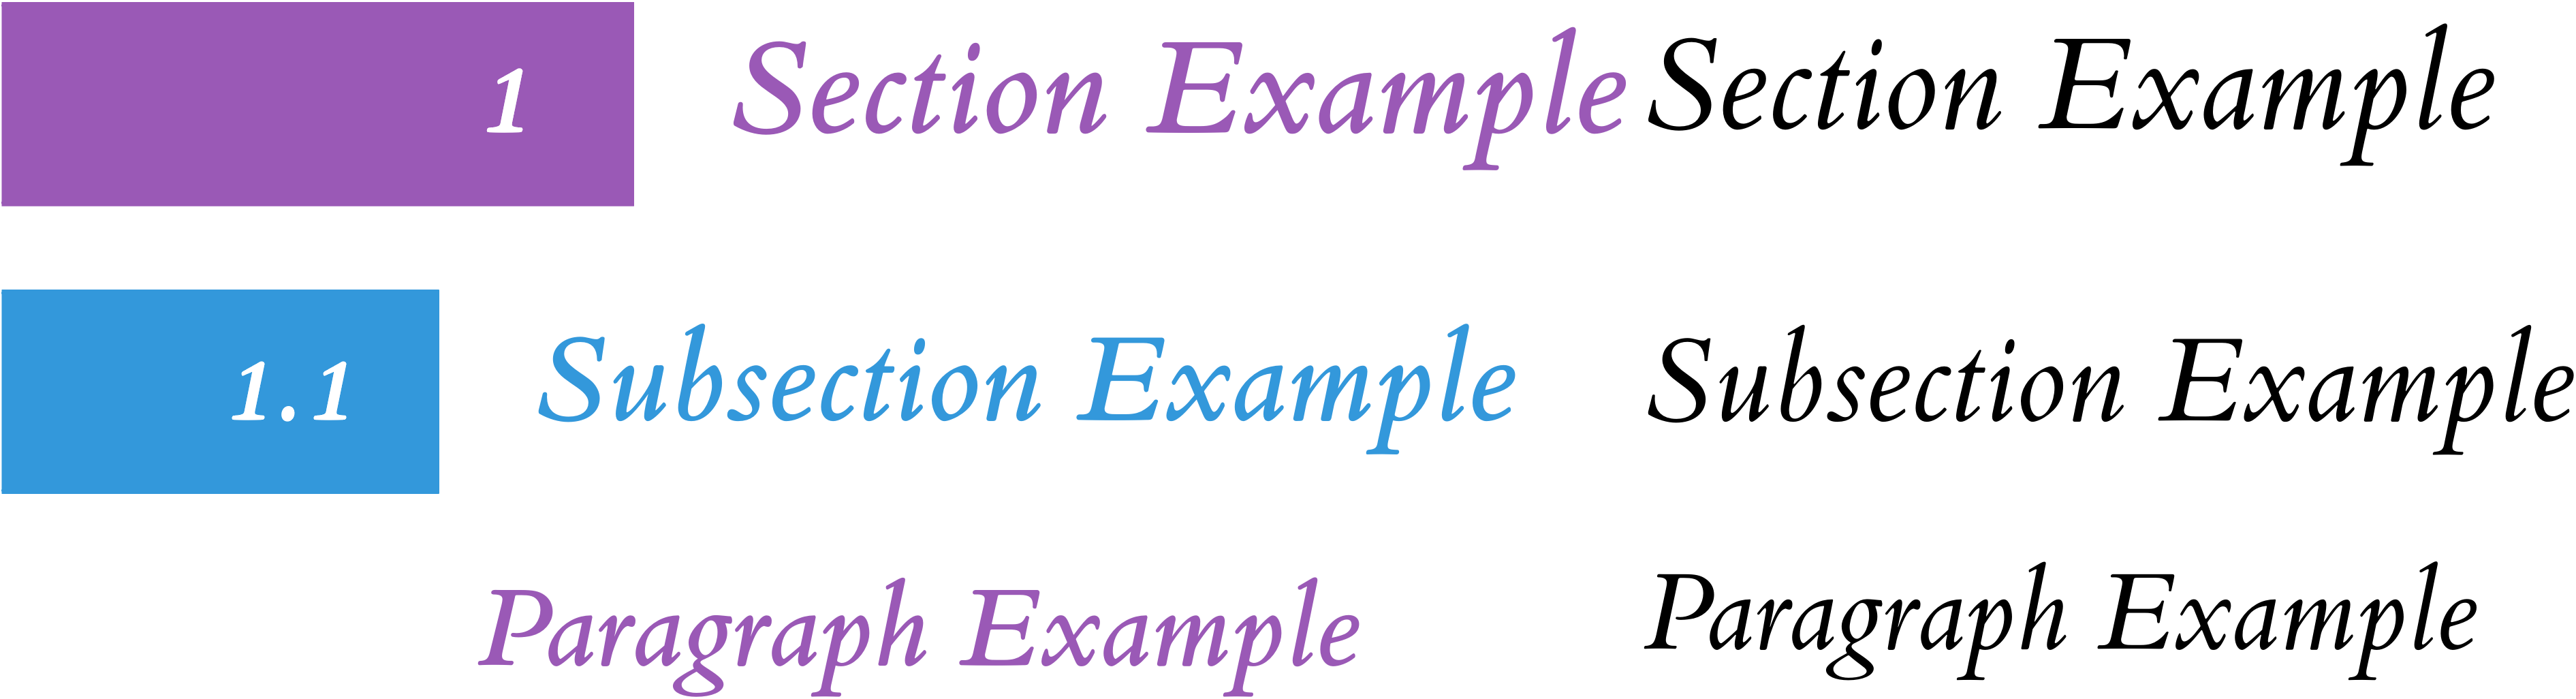
\includegraphics{section-comparison.png}
  \caption[Comparison between modern and old section styles]{%
    Comparison between modern and old style section headings.
    \emph{Notice that the spacing between the sections is a little bit different.}
    \emph{This was motivated by wanting to equalize the spacing between colored boxes.}
  }\label{fig:section-headings}
\end{figure*}


\section{Compatibility Issues}\label{ch:compatibility}
When switching an existing document from one document class to a \TL\ document class, a few changes to the document may have to be made.


\subsection{Converting from \doccls{article} to \doccls{tufte-handout}}\label{sec:article-to-handout}
The following \doccls{article} class options are unsupported: \docclsopt{10pt}, \docclsopt{11pt}, \docclsopt{12pt}, \docclsopt{a5paper}, \docclsopt{b5paper}, \docclsopt{executivepaper}, \docclsopt{legalpaper}, \docclsopt{landscape}, \docclsopt{onecolumn}, and \doccls{twocolumn}.

The following headings are not supported: \doccmd{subsubsection} and \doccmd{subparagraph}.


\subsection{Converting from \doccls{book} to \doccls{tufte-book}}\label{sec:book-to-tufte-book}
The following \doccls{book} class options are unsupported: \docclsopt{10pt}, \docclsopt{11pt}, \docclsopt{12pt}, \docclsopt{a5paper}, \docclsopt{b5paper}, \docclsopt{executivepaper}, \docclsopt{legalpaper}, \docclsopt{landscape}, \docclsopt{onecolumn}, and \doccls{twocolumn}.

The following headings are not supported: \doccmd{subsubsection} and \doccmd{subparagraph}.


\section{Troubleshooting and Support}\label{ch:troubleshooting}
\subsection{\TL\ Website}\label{sec:website}
The original website for the \TL\ packages is located at \url{https://tufte-latex.github.io/tufte-latex/}.
On that website, you'll find links to the \smallcaps{git} repository, mailing lists, bug tracker, and documentation.

However as the project seems to be abandoned as of time of writing, the website may not be available in the future.
Additionally some of the links there seem to have already been victim of link rot.
You can find more help and information on the current development of the \TL\ classes at my GitHub repository.
\url{https://github.com/MormonJesus69420/Modernized-Tufte-LaTeX}

\TODO{Create a new website for the project and link it here}


\subsection{\TL\ Mailing Lists}\label{sec:mailing-lists}
There is only one surviving mailing list for the \TL\ project:

\paragraph{Discussion list}
The \texttt{tufte-latex} discussion list is for asking questions, getting assistance with problems, and help with troubleshooting. 
Release announcements were also posted to this list.%
\marginnote{You can subscribe to the \texttt{tufte-latex} discussion list at \url{http://groups.google.com/group/tufte-latex}}

\paragraph{Commits list}
The \texttt{tufte-latex-commits} list used to exist as well as a read-only mailing list. 
Messages were sent to the list any time the \TL\ code had been updated.%
\marginnote{This list was available at \url{http://groups.google.com/group/tufte-latex-commits}}

A more modern way to keep up with the development of the \TL\ classes is to follow the GitHub repository.
You can use the \textit{Discussions} feature to ask questions, suggest improvements, and interact with other users.%
\marginnote{\url{https://github.com/MormonJesus69420/Modernized-Tufte-LaTeX/discussions}}
In case you notice and bugs with the classes, or notice any issues with the documentation, you can open an issue on the GitHub repository.%
\marginnote{\url{https://github.com/MormonJesus69420/Modernized-Tufte-LaTeX/issues}}
In case you want to contribute to the project, you can open a pull request on the GitHub repository.%
\marginnote{\url{https://github.com/MormonJesus69420/Modernized-Tufte-LaTeX/pulls}}

\newthought{I don't plan on using mailing lists} in my project, as I never got used to them, and feel that GitHub provides a more user friendly way to interact with the project.


\subsection{Getting Help}\label{sec:getting-help}
If you've encountered a problem with one of the \TL\ document classes, have a question, or would like to report a bug, please create an issue or start a discussion on the GitHub repository.

To help with troubleshooting the problem more quickly, please try to compile your document using the \docclsopt{debug} class option.
When asking for help include the generated \texttt{.log} file in the issue, along with a brief description of the problem, and if possible a minimal working example that reproduces the issue.
You can also upload your whole document if you're not sure what's causing the issue, and you are comfortable with sharing the document.


\subsection{Package Dependencies}\label{sec:dependencies}
The following is a list of packages that the \TL\ document classes rely upon. 
Packages marked with an asterisk are either optional or only loaded for some class options.
\begin{multicols}{2}
  \begin{itemize}
    \item ams\{math,symb,thm,xtra\} * \textit{for \texttt{Note} environments}
    \item biblatex * \textit{only if \texttt{nobib} is off, requires \texttt{biber} backend}
    \item bidi * \textit{only if using \texttt{bidi} option}
    \item changepage
    \item chngpage * \textit{only if \texttt{changepage} is not available}
    \item cleveref * \textit{for \texttt{Note} environments}
    \item ETbb * \textit{if available, and \texttt{nofonts} is off}
    \item fancyhdr
    \item FiraMono * \textit{if available, and \texttt{nofonts} is off}
    \item fontenc * \textit{only with \iPdfLaTeX, and \texttt{nofonts} is off}
    \item fontspec * \textit{only with \iXeLaTeX\ or \iLuaLaTeX, and \texttt{nofonts} is off}
    \item geometry
    \item gillius2 * \textit{if available, and \texttt{nofonts} is off}
    \item hardwrap
    \item hyperref * \textit{only if \texttt{nohyper} is off}
    \item iftex * \textit{if not it assumes \hologo{pdfLaTeX}}
    \item letterspace * \textit{only if \texttt{nols} is off}
    \item mathpazo * \textit{if available, and \texttt{nofonts} is off}
    \item multicol
    \item optparams
    \item paralist
    \item placeins
    \item ragged2e
    \item sectsty
    \item setspace
    \item soul * \textit{only with \hologo{pdfLaTeX}}
    \item textcase
    \item textcomp * \textit{only with \hologo{pdfLaTeX}, and \texttt{nofonts} is off}
    \item thmtools * \textit{for \texttt{Note} environments}
    \item titlesec
    \item titletoc
    \item transparent
    \item xcolor
    \item xifthen
    \item xkeyval
  \end{itemize}
\end{multicols}

\subsection{More Documentation}\label{sec:more-doc}
For more documentation on the Tufte-\LaTeX{} document classes (including commands not
mentioned in this handout), please see the sample book.

\subsection{Support}\label{sec:support}

The website for the Tufte-\LaTeX\ packages is located at
\url{https://github.com/Tufte-LaTeX/tufte-latex}. On our website, you'll find
links to our \smallcaps{svn} repository, mailing lists, bug tracker, and documentation.

% Print Bibliography
\printbibliography[heading=bibnumbered]

\end{document}
